\documentclass{llncs}
\usepackage[utf8]{inputenc}
\usepackage{llncsdoc}
\usepackage{graphicx}
\usepackage{hyperref}
\usepackage{listings}
\usepackage{color}

\newcommand{\inlinecode}{\texttt}

\begin{document}

\title{Fault Tolerance for PCJ}

\author{Michał Szynkiewicz}
\institute{Faculty of Mathematics and Computer Science Nicolaus Copernicus University, Toruń, Poland}

\date{2015}
\maketitle

\begin{abstract}

Nowadays, distributed computations are often run on large amounts of nodes for a significant amount of time.
Having a 24 hour long computation on 1000 nodes means almost 3 years of computations.
As calculated in \cite{rx10}, with 6 month mean time between failures, it gives less than 1\% chance of success.

PCJ library is a high-performance parallel computing library for Java implementing PGAS model.

This paper describes changes introduced in PCJ to provide basic fault tolerance and fault tolerance strategies that are planned to be implemented in future.

\end{abstract}

\section{Introduction}
Before the changes described in this paper, any network or hardware failure resulted in hanging of a PCJ-based program.

The changes introduce \emph{Ignore failure} fault tolerance policy.
This is a minimum-overhead, no-checkpoint strategy.

For programs that do not require results from all nodes to finish, like Monte Carlo randomized algorithms, the strategy is enough to finish calculations properly.
For others, the strategy provides a useful base on which the programmer may build a dedicated solution (e.g. replaying failed nodes work on other node).



\section{PCJ library overview}
PCJ library is an implementation of PGAS model.
The smallest unit of computation is called a \emph{thread}. Each \emph{thread} has its own local address space and shared address space.
The owner thread accesses local and global address spaces variables as usual Java fields.
Following is a description of PCJ features. For more details please see \cite{pcj-manual}.
\subsection{Synchronization}
Threads synchronization in PCJ is realized by \inlinecode{barrier}.
Barrier can be made either across all threads or two threads.
In first case each task has to call \inlinecode{barrier} method.
\subsection{Shared memory}
Fields that should be put into shared address space have to be annotated in \inlinecode{@Shared} annotation.
Aformentioned fields are accessible from other threads via following methods:
\begin{itemize}
\item\inlinecode{get(threadId, variableName)}, \inlinecode{getFutureObject(threadId, variableName)} - read the value of given variable
in a synchronous and asynchronous fashion
\item\inlinecode{put(threadId, variableName, value)} - asynchronously update variable value on given node.
\item\inlinecode{broadcast(variableName, value)} - asynchronously update variable value on all nodes.
\end{itemize}
\inlinecode{waitFor(variableName)} and \inlinecode{monitor(variableName)} can be used to lock the current thread until other thread updates given variable on this node.



% mstodo move to the bottom, describe current solution?
%\section{Concepts}
%Currently we assume that there is a special node, namely \textit{node 0}, that never dies.
%We plan to provide two fault tolerance strategies: ignoring node failure and respawning failed threads.
%  \\
%Moreover we plan to provide a resilient storage to make it possible to restore thread state from a snapshot.
%Resilient storage will have two modes: synchronous and asynchronous.
%Synchronous mode will allow programs to recover from the latest position achieved by the failed thread.
%In asynchronous mode state will be saved in a storage in a non-blocking fashion.
%\\
%                \\
%%                mstodo: move descriptions elsewhere
%\section{Example use cases of strategies}
%Following are examples of possible usages of fault tolerance strategies described in this paper.
%\subsection{Ignore failure}
%The failed node is ignored, all of its' data is lost.
%Might be used for instance for monte carlo randomized algorithms, e.g. monte carlo Pi approxmiation.
%\subsection{Respawn node with synchronous resilient storage}
%The most powerful strategy. Upon failure of physical node all the threads running on it are recreated on other nodes.
%Then the state of threads is recreated from the latest saved state.
%Might be used for example for parallel FFT implementation.
%In FFT implementation, in multiple phases, each thread first makes computations and then broadcasts the results.
%It is crucial to remember the exact state from the broadcasting phase.
%% mstodo: verify
%\subsection{Respawn node with asynchronous resilient storage}
%As in previous strategy, threads are recreated on active nodes.
%The state is restored from resilient storage, but since the storage is asynchronous, it might contain old data.

\section{API}
The main concern for the API changes provided by the implementation is not to break

\subsection{Impact on API}

\section{Node failure handling implementation}

The main elements of implementation are: monitoring nodes for failure and adjusting configuration after node failure.

\subsection{Node monitoring}
Monitoring works in two ways::
\begin{itemize}
\item The immortal \textit{node 0} is monitoring other nodes by sending PING message and waiting for PONG.
If, for some node, sending PING fails, or the node does not answer with PONG for a long (configurable) time,
it is assumed failed. Please see Fig. \ref{pinging} \nameref{pinging}.
\item
If \textit{node A} encounters a communication error when trying to communicate with \textit{node B}
(e.g. if updating a variable value on \textit{node B} fails), \textit{node A} informs \textit{node 0} that \textit{node B} has failed.

\end{itemize}

\begin{figure}
  \centering
      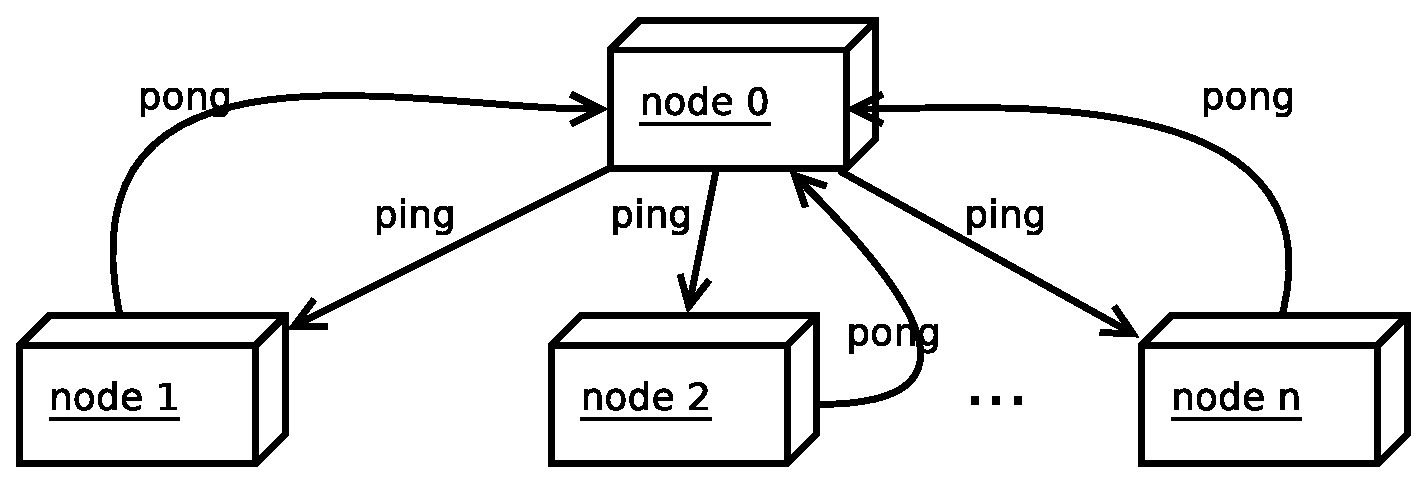
\includegraphics[width=0.5\textwidth]{node-monitoring.eps}
  \caption{Node monitoring}
  \label{pinging}
\end{figure}

\subsection{Reconfiguration}
On node failure \textit{node 0} sends a proper reconfiguration message to all nodes.
Depending on the type of selected strategy there are two...

\section{Performance overhead}

\section{Resilient storage implementation}

\section{Future plans}

\section{Conclusion}

\begin{thebibliography}{1}

\bibitem{rx10}
Leslie Lamport, Dave Cunningham, Dave Grove, Ben Herta, Arun Iyengar, Kiyokuni Kawachiya, Hiroki Murata, Vijay Saraswat, Mikio Takeuchi, Olivier Tardieu
\emph{Resilient X10. Efficient failure-aware programming},
19th ACM SIGPLAN Symposium on Principles and Practice of Parallel Programming, Orlando, Florida, 2014, Lecture
\bibitem{pcj}
Marek Nowicki, Piotr Bała
\emph{PCJ - New Approach for Parallel Computations in Java}
Applied Parallel and Scientific Computing, 11th International Conference, PARA 2012, Helsinki, Finland, June 10-13, 2012, Revised Selected Papers
% mstodo how to cite it properly?
\bibitem{pcj-manual}
Marek Nowicki, Piotr Bała
\emph{PCJ. Parallel Computing in Java}, 2013, [Online]. Available: \url{http://pcj.icm.edu.pl/c/document_library/get_file?uuid=e8b5a416-644d-43d0-a19c-74e14555ef96&groupId=43801} [2015, April 14]

\end{thebibliography}

\end{document}
